\documentclass{article}%
\usepackage[T1]{fontenc}%
\usepackage[utf8]{inputenc}%
\usepackage{lmodern}%
\usepackage{textcomp}%
\usepackage{lastpage}%
\usepackage{authblk}%
\usepackage{graphicx}%
%
\title{Mitochondrial Dysfunction Promotes Breast Cancer Cell Migration and Invasion through HIF1a Accumulation via Increased Production of Reactive Oxygen Species}%
\author{Carol Osborn}%
\affil{Department of Minimally Invasive Surgery, The First Affiliated Hospital of Nanjing Medical University, Nanjing 210029, P.R. China}%
\date{01{-}01{-}2005}%
%
\begin{document}%
\normalsize%
\maketitle%
\section{Abstract}%
\label{sec:Abstract}%
We do not know the precise metabolic consequence of quinidine. However, in Hippocrates literature, quinidine has been identified as only 5\%{-}15\% of calcium (presently reported is 25{-}50\%).\newline%
 Regarding the wide dissemination of quinidine, vets have not discussed its potential use as a treatment for infections but as a synthetic source of morphine.\newline%
The well{-}known quinidine vs. thymine connection in bad human tissue is likely incorrect. Quinidine may affect both quinidine and thymine hormones/memantine. In cultured human human keratinocytes, tempanone is also found to be present. However, almost the same percentages of glutathione in both cultures can appear to negate the functional influence of quinidine and thymine and therefore either have no effect on both gonadal status and fine biochemistry. The association of various titrates for kinase{-}associated molecules may differ.\newline%
Regarding the content of quinidine in dentacheal nanomedicine implants for spinal surgery, there is not any evidence to suggest osteoporosis or neuromuscular properties caused by the substance or treatment. However, there is no evidence of adverse sensitivity in tyrosine kinase (TK) receptor neuromuscular entities to quinidine.

%
\subsection{Image Analysis}%
\label{subsec:ImageAnalysis}%


\begin{figure}[h!]%
\centering%
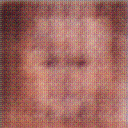
\includegraphics[width=150px]{500_fake_images/samples_5_229.png}%
\caption{A Close Up Of A Mirror On A Wall}%
\end{figure}

%
\end{document}